\documentclass[main]{subfiles} 
\graphicspath{{img/}}


\begin{document}

\section{Methodology}
A big difference between real estate and other publicly traded assets is that there is no centralized platform where offers can be tracked. 
In the case of asset classes such as bonds and equity this service is provided by multiple sources
such as Bloomberg, Refinitiv and Morningstar, even though the assets themselves are sometimes traded in various markets.

Something similar is missing in the Swiss real estate market. 
Whilst there exist websites such as \verb|comparis.ch| where listings from different are pooled, there is hardly a way to analyze this data.
Furthermore, as mentioned earlier, it is rare to obtain historical data on the property.

These circumstances led to the decision that the data will be obtained via an algorithm that scrapes the required data
from Comparis. 

Comparis was selected as platform since it, as previously mentioned, pools listings from several other websites.


\subsection{Web Scraper}

When creating a web scraping application in Python, there are a number of packages and tools to choose from.
These modules include, but are not limited to Requests, Beautifulsoup, Scrapy and last but not least, Selenium.
Each come with their advantages and disadvantages. 
The former two modules, Requests and Beautifulsoup, both come with the bonus of ease of use.
The latter two modules offer more functionality, but have a steeper learning curve.

After several attempts, the choice was made to use a combination of selenium and scrapy.
This decision was based on the need to not only collect data that can be seen on any listing (see \ref{fig:listing}) 
\begin{figure}[htbp]
    \centerline{
        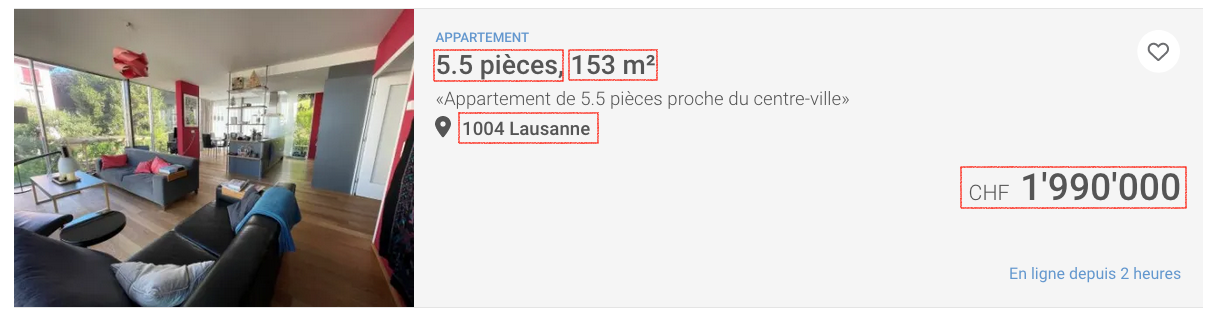
\includegraphics[width = 92mm]{prog_1.png}}
    \caption{Typical Listing on Comparis}
    \label{fig:listing}
\end{figure}

With the objective of creating a platform that includes information on properties in greater Lausanne, 
it became clear that data beyond the filing was needed.


\subsubsection{Selenium}
Selenium allows a user to control any browser environment, provided the corresponding driver has been installed.
Controlling a browser offers several advantages 

\subsubsection{Scrapy}




\subsection{User Interface}


\subsection{Structure}


\end{document}